\documentclass{article}

\usepackage{amsmath, amsthm, amssymb, amsfonts}
\usepackage{thmtools}
\usepackage{graphicx}
\usepackage{setspace}
\usepackage{geometry}
\usepackage{float}
\usepackage{hyperref}
\usepackage[utf8]{inputenc}
\usepackage[english]{babel}
\usepackage{framed}
\usepackage[dvipsnames]{xcolor}
\usepackage{tcolorbox}
\usepackage{booktabs}
\usepackage{caption}
\usepackage{subcaption}
\usepackage{listings}

\newcommand{\HRule}[1]{\rule{\linewidth}{#1}}

\newcommand{\dsanote}[1]{\textbf{[dsa: #1]}}

% ------------------------------------------------------------------------------

\begin{document}

% ------------------------------------------------------------------------------
% Cover Page and ToC
% ------------------------------------------------------------------------------

\title{ \normalsize \textsc{}
		\\ [2.0cm]
		\HRule{1.5pt} \\
		\LARGE \textbf{Parallel and Distributed Computing
		\HRule{2.0pt} \\ [0.6cm] \LARGE{Project Report - MPI Delivery} \vspace*{10\baselineskip}}
		}
\date{}
\author{\textbf{Authors} \\ 
		Carolina Coelho - 99189\\
		Diogo Melita - 99202\\
		Diogo Antunes - 99210}
\maketitle
\newpage

% ------------------------------------------------------------------------------

\section{Introduction}

The goal for this stage is to parallelize the serial version of the \texttt{lifed3d} 
program using MPI.

\section{MPI Approach}

In the \texttt{OpenMP} phase, it was already established which part of the code needed parallelization. 
In this stage, this work will be split among processes instead of a team of threads.

\subsection{Data Decomposition}

The initial step in this stage involved determining how the grid would be divided among the various machines.
Three decompositions were considered - decomposition along the x axis into slices,
along the x and y axis and along all axis. A visualization of the different approaches
can be found in Figure~\ref{fig:viz-decomp}.

\begin{figure}[ht]
    \centering
    \begin{subfigure}[b]{0.2\textwidth}
      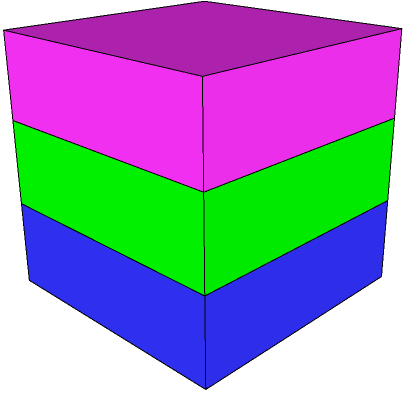
\includegraphics[width=\textwidth]{img/decomp-1.png}
      \caption{Approach A: x-axis decomposition (slicing)}
      \label{subfig:a}
    \end{subfigure}
    \hfill
    \begin{subfigure}[b]{0.2\textwidth}
      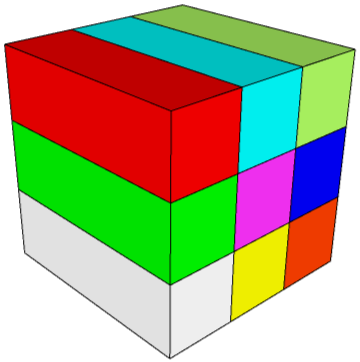
\includegraphics[width=\textwidth]{img/decomp-2.png}
      \caption{Approach B: x and y-axis decomposition}
      \label{subfig:b}
    \end{subfigure}
    \hfill
    \begin{subfigure}[b]{0.2\textwidth}
      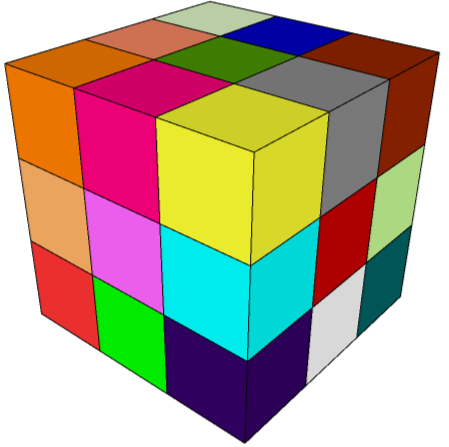
\includegraphics[width=\textwidth]{img/decomp-3.png}
      \caption{Approach C: all axis decomposition (checkerboard)}
      \label{subfig:c}
    \end{subfigure}
    \caption{Different grid decompositions}
    \label{fig:viz-decomp}
\end{figure}

For a fixed number of CPUs, the computation performed in total will be the same.
For division B to be possible, $p$ (the number of processes) must be a product
of 2 non-trivial factors and for C, the number must be a product of 3 non-trivial factors.
Let us assume that $p = a \times b \times c$, with $a \ge b \ge c$. 
The expected communication will be $2n^2$,  $2an + 2bcn$ and
$2ab + 2ac + 2bc$ cells, respectively. To better understand what this means,
let't consider $p=64=4^3$. The expected communication will be $2n^2$,
$4 \times (\frac{n}{4}n)^2 = \frac{n^2}{4}$ and $6 \times (\frac{n}{4}\frac{n}{4})^2 = \frac{3n}{128}$
cells, respectively.

This means that the division against more dimensions further reduces communication.
However, it is also clear that the division in more than one dimension is also
much more complex and error-prone (also, it would require more calls to \texttt{ISend}
and \texttt{IRecv}, because only a y-z layer is stored contiguously in memory).
For this reason, our approach was to implement first division A and if communication
proved to be a bottleneck move to more complex grid divisions.

Since instances might be too large to fit into a single machine's memory, each
machine only stores its piece of the map. For each generation, each process will
only compute the statistics for the stored part of the map and at the end the master
root process aggregates all the results and updates the global statistics.
Given the partitioning chosen, each machine needs only to 
communicate with the adjacent machines. During this 
communication, the involved machines would exchange their borders - the leftmost
and rightmost slices of the node's piece of the grid.

% This approach led to the decision that each machine would only need to allocate resources for the 
% slice it was assigned, effectively reducing the program's memory usage on each machine. Following 
% the grid partitioning, the next crucial step was determining how communication between the machines 
% would be managed. Given the horizontal partitioning of the grid, each machine would only need to 
% communicate with the adjacent machines—specifically, the previous and next machines. During this 
% communication, the involved machines would exchange their borders, as these are necessary for 
% computing the next generation of border cells.


\subsection{Implementation}

In the first implementation, at the start of each generation, each node computes
the new values for the current grid (and while doing this, computes the new
statistics), then exchanges with the neighbors the new border values (using the asynchronous
communication primitives \texttt{ISend} and \texttt{IRecv}). At the end of the
exchange, the machine-local statistics are aggregated at the root machine (using \texttt{Reduce}).
It should be noted that a single \texttt{ISend} and \texttt{IRecv} are done per layer,
which is possible because the y-z-plane is store contiguously in memory (this isn't possible
for any other plane, in particular for any other data decomposition, the number of calls will
grow with $n$).

This division already achieved very good speedups, specially for large values of 
$n$. In particular, for the 4 inputs considered, the execution time breakdown can
be found in Figure~\ref{time-breakdown}.
(the raw data is provided in Appendix A, Table~\ref{tab:mpi_performance})

\begin{figure}[htbp]
    \centering
    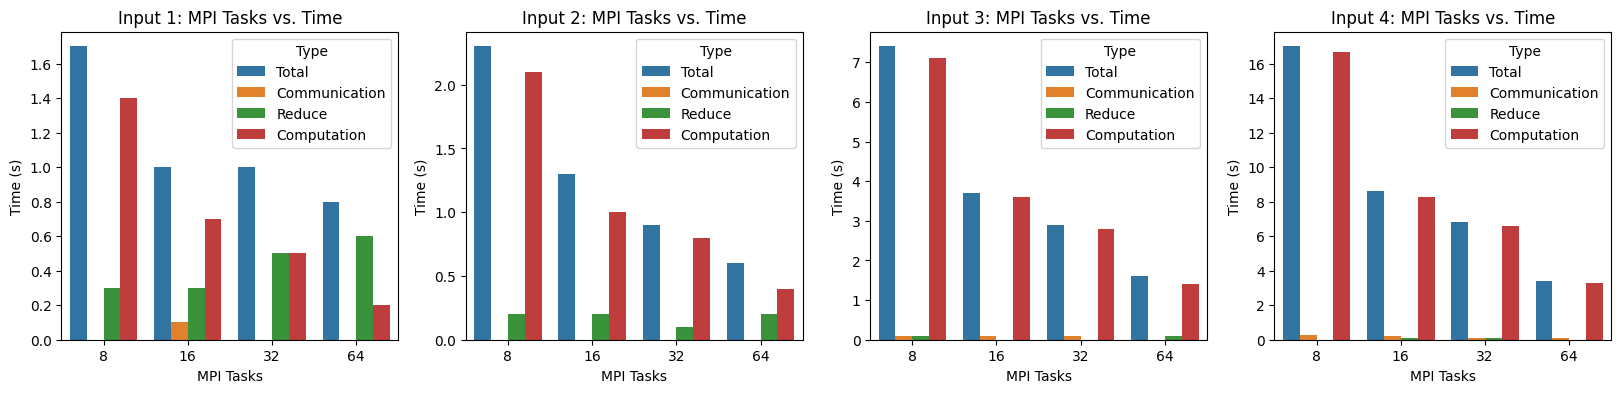
\includegraphics[width=1\textwidth]{img/first-version-breakdown.png}
    \caption{Execution time breakdown for first version}
    \label{time-breakdown}
\end{figure}

The results show that computation is the bottleneck across all settings, which means that
the parallelization overhead is small. However, it is
clear that for small values of $n$, the reduction time is also considerable. The key insight
is that this reduction can be done while the computation of the new grid takes place.
To do this, \texttt{Reduce} was 
replaced by its asynchronous counterpart - \texttt{IReduce}. A small caveat is that
two local statistics arrays are required - one for the old statistics, over which the 
reduction is working and one to store the statistics regarding the new grid state.
In summary, with this approach, each node performs the following steps:

\begin{enumerate}
	\itemsep -0.2em
	\item compute the new state of its part of the grid
	\item share borders (using \texttt{ISend} and \texttt{IRecv})
	\item wait for previous reduction (using \texttt{Wait})
	\item update the problem solution (root node only) 
	\item wait for border exchange to complete (using \texttt{WaitAll})
	\item start new reduction (using \texttt{IReduce})
\end{enumerate}

An alternative implementation was developed, where the border exchange process
was done in background, while the computation of the "core" layers was performed.
Since the communication is not be the biggest overhead, no meaningful speedup
was expected. The code and the results, which confirm the expectation, can be found
in Appendix B.

\subsection{Load balancing}

In the partitioning scheme chosen, the load for two nodes differs by at most
a single layer. Given the values of $n$ and $p$ considered, one always represents
a small percentage of the overall workload. The biggest problem in terms of load balancing
was found when testing the solution
in multiple labs. The lab's machines computing power is not uniform across
the cluster and when different labs are used simultaneously, the homogeneous work division
didn't prove to be the best, since the fastest machines had to wait for the slowest in the group.
A solution to
this would be to have dynamic division of work - for example, at the end
of each round, every node could compare with its neighbors the time it took to finish
the computation. If the difference was above some threshold, the fastest
neighbor would steal some of the work. This solution was already
out of the scope of the project, so it was not implemented.

\section{Hybrid approach}

Besides the MPI-only, a hybrid approach was also implemented.
As already seen, the communication didn't prove to be much of an overhead, so
no extra speedup was expected from this version. The approach to extending the MPI
solution to a hybrid one resembles the one used to parallelize the initial
serial version. A team of threads is spawned at the start of MPI instance (using
the \texttt{omp parallel} pragma). The computation of the new state of the replica's
slice is divided among the threads (using \texttt{omp for}) and all remaining tasks
(border exchange and reduction) are executed only by the master threads, which is
achieved using \texttt{omp single}.

\section{Experimental results}

\subsection{MPI}

The final solution was benchmarked in RNL lab2 machines against the four public
test provided by the faculty team. The results for the MPI only version 
(\texttt{OMP\_NUM\_THREADS = 1}) is presented in tables \ref{execution-times} and
\ref{speedup}.

\begin{table}[h!]
	\centering
	\begin{tabular}{||c c c c c c||} 
	 \hline
	 Version & \#Nodes & Input 1 & Input 2 & Input 3 & Input 4\\ [0.5ex] 
	 \hline\hline
	 serial & $N/A$ & 13.2 & 20.8 & 72.5 & 168.1 \\ 
	 MPI & 8 & 1.8 & 2.3 & 7.2 & 16.9 \\ 
	 MPI & 16 & 0.9 & 1.2 & 3.9 & 8.5  \\
	 MPI & 32 & 0.7 & 0.9 & 2.9 & 6.8 \\
	 MPI & 64 & 0.4 & 0.5 & 1.5 & 3.7 \\ [1ex] 
	 \hline
	\end{tabular}
	\caption{Times of execution, in seconds, of the serial and parallelized versions of the code.}
	\label{execution-times}
\end{table}

\begin{table}[h!]
	\centering
	\begin{tabular}{||c c c c c||} 
	 \hline
	 \#Nodes & Input 1 & Input 2 & Input 3 & Input 4\\ [0.5ex] 
	 \hline\hline
	 8 & 7.3 & 9 & 10.1 & 9.9 \\ 
	 16 & 14.7 & 17.3 & 18.6 & 19.8  \\
	 32 & 18.9 & 23.1 & 25 & 24.7 \\
	 64 & 33 & 41.6 & 48.6 & 45.4 \\ [1ex] 
	 \hline
	\end{tabular}
	\caption{Speedup achieved with the parallelized versions of the code, comparing to the serial version}
	\label{speedup}
\end{table}

\begin{figure}[htbp]
    \centering
    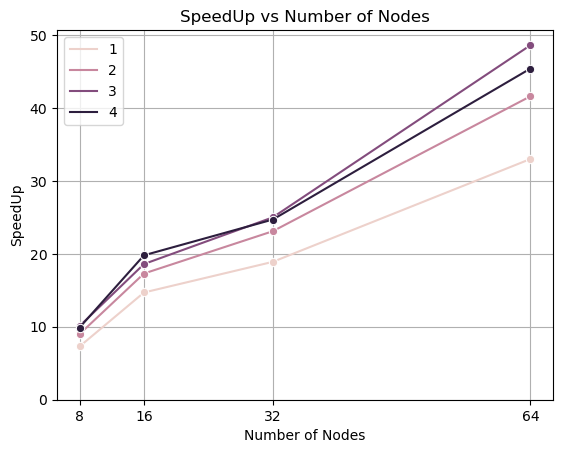
\includegraphics[width=0.5\textwidth]{img/speedup.png}
    \caption{Speedup achieved by the parallelized version when running on different number of nodes.}
    \label{speedup-graph}
\end{figure}

The results for Input 2 through 4 are rather surprising, since for 8 and 16 nodes
the speedup is \textbf{greater than} the ideal speedup. This can be explained
by a reduction of the total computation required. The serial version must perform a
wrap-around in all three dimensions (and for this it requires modular arithmetic).
Since the MPI program keeps the
previous and next layer, modular arithmetic only needs to be performed in two
dimensions, which means there's a reduction in the computation required. To test this hypothesis,
the original serial program was changed in the following way (this
obviously breaks the code, the goal is just to evaluate the impact of removing the
two division operations):

\begin{lstlisting}[language=C,caption={Change to serial code}]
// int32_t left = (x - 1 + n) % n;
int32_t left = x;
// int32_t right = (x + 1 + n) % n;
int32_t right = x;
\end{lstlisting}

The comparison between MPI with a single process, the serial unaltered version
and the serial altered version can be found in Table~\ref{tbl:serial-times}.
Even though the results for MPI with $n=1$ don't perfectly match the altered serial
version, it is clear that a large part of the super-linear speedup can be explained
by the reduction of the required computation due to program design changes.

This example shows that in this stage of the project multiple (sometimes unexpected)
factors impact the overall performance (other factors could be mentioned, such as the
fact that at some point processes are hosted in different machines, thereby increasing
communication latency). Since this is the case, making comparisons against theoretical estimations is
less objective.
For this reason, in this report, unlike the previous one, Amdahl's law or other metrics
mentioned in the lectures are not used to verify the experimental results against
concrete theoretical predictions.

\begin{table}[h!]
	\centering
	\begin{tabular}{||c c c c||} 
	 \hline
	 Input & MPI with $n=1$ & Serial unaltered & Serial altered \\ [0.5ex] 
	 \hline
	 1 & 10.8 & 13.4 & 11.9 \\  [1ex] 
	 2 & 17.2 & 21.3 & 18.9 \\  [1ex] 
	 3 & 57.7 & 69.3 & 58.4 \\  [1ex] 
	 4 & 136.4 & 160.1 & 136.9 \\  [1ex] 
	 \hline
	\end{tabular}
	\caption{Times of execution, in seconds, of several serial versions}
	\label{tbl:serial-times}
\end{table}

\subsection{Hybrid approach}

A hybrid MPI+OpenMP approach using 16 processes each with 4 threads was compared with a 64 process
MPI solution and the results are presented in Table~\ref{tbl:hybrid-results}. As already mentioned, since the results show that computation
is the bottleneck, no improvement is expected, and the results confirm this expectation
(there's even a very slight degradation, likely due to the extra
synchronization required).

\begin{table}[h!]
	\centering
	\begin{tabular}{||c c c c c c c||} 
	 \hline
	 Version & Number of Nodes & Number of Threads & Input 1 & Input 2 & Input 3 & Input 4\\ [0.5ex] 
	 \hline\hline
	  MPI+OMP & 16 & 4 & 0.5 & 0.6 & 1.7 & 3.8 \\  [1ex] 
	 \hline
	  MPI & 64 & 1 & 0.4 & 0.5 & 1.5 & 3.7 \\  [1ex] 
	 \hline
	\end{tabular}
	\caption{Times of execution, in seconds, of the hybrid version and corresponding MPI version}
	\label{tbl:hybrid-results}
\end{table}

\newpage

\section{Appendix A}

\begin{table}[htbp]
  \centering
  \begin{tabular}{lcccc}
    \toprule
    \textbf{Number of tasks} & \textbf{Total time (s)} & \textbf{Communication (s)} & \textbf{Reduce (s)} & \textbf{Computation (s)} \\
    \midrule
    \textbf{Input 1} & & & & \\
    8 MPI Tasks & 1.7 & 0.0 & 0.3 & 1.4 \\
    16 MPI Tasks & 1.0 & 0.1 & 0.3 & 0.7 \\
    32 MPI Tasks & 1.0 & 0.0 & 0.5 & 0.5 \\
    64 MPI Tasks & 0.8 & 0.0 & 0.6 & 0.2 \\
    \midrule
    \textbf{Input 2} & & & & \\
    8 MPI Tasks & 2.3 & 0.0 & 0.2 & 2.1 \\
    16 MPI Tasks & 1.3 & 0.0 & 0.2 & 1.0 \\
    32 MPI Tasks & 0.9 & 0.0 & 0.1 & 0.8 \\
    64 MPI Tasks & 0.6 & 0.0 & 0.2 & 0.4 \\
    \midrule
    \textbf{Input 3} & & & & \\
    8 MPI Tasks & 7.4 & 0.1 & 0.1 & 7.1 \\
    16 MPI Tasks & 3.7 & 0.1 & 0.0 & 3.6 \\
    32 MPI Tasks & 2.9 & 0.1 & 0.0 & 2.8 \\
    64 MPI Tasks & 1.6 & 0.0 & 0.1 & 1.4 \\
    \midrule
    \textbf{Input 4} & & & & \\
    8 MPI Tasks & 17.0 & 0.3 & 0.0 & 16.7 \\
    16 MPI Tasks & 8.6 & 0.2 & 0.1 & 8.3 \\
    32 MPI Tasks & 6.8 & 0.1 & 0.1 & 6.6 \\
    64 MPI Tasks & 3.4 & 0.1 & 0.0 & 3.3 \\
    \bottomrule
  \end{tabular}
  \caption{First version execution time breakdown}
  \label{tab:mpi_performance}
\end{table}

\newpage

\section{Appendix B}

\begin{table}[htbp]
  \centering
  \caption{MPI with background border exchange performance summary}
  \label{tab:mpi_performance_bg}
  \begin{tabular}{lc}
    \toprule
    \textbf{Input} & \textbf{Execution time (seconds)}\\
    \midrule
    \textbf{1} & \\
    8 MPI Tasks & 1.7 \\
    16 MPI Tasks & 1.1 \\
    32 MPI Tasks & 0.7 \\
    64 MPI Tasks & 0.5 \\
    \midrule
    \textbf{2} & \\
    8 MPI Tasks & 2.2 \\
    16 MPI Tasks & 1.7 \\
    32 MPI Tasks & 0.9 \\
    64 MPI Tasks & 0.5 \\
    \midrule
    \textbf{3} & \\
    8 MPI Tasks & 7.3 \\
    16 MPI Tasks & 5.7 \\
    32 MPI Tasks & 2.9 \\
    64 MPI Tasks & 1.5 \\
    \midrule
    \textbf{4} & \\
    8 MPI Tasks & 17.1 \\
    16 MPI Tasks & 13.5 \\
    32 MPI Tasks & 7.3 \\
    64 MPI Tasks & 3.4 \\
    \bottomrule
  \end{tabular}
\end{table}


\begin{lstlisting}[language=C,caption={Generation loop for background exchange of borders}]
for (int32_t gen = 0; gen < max_gen; gen++) {
  for (int32_t y = 0; y < n; y++) {
    for (int32_t z = 0; z < n; z++) {
      new_val = next_inhabitant(1, y, z, n, old);
      new[1][y][z] = new_val;
      population_local[new_val]++;
    }
  }

  if (height > 1) {
    for (int32_t y = 0; y < n; y++) {
      for (int32_t z = 0; z < n; z++) {
	new_val = next_inhabitant(height, y, z, n, old);
	new[height][y][z] = new_val;
	population_local[new_val]++;
      }
    }
  }

  computation_time += MPI_Wtime();
  total_computation_time += computation_time;

  // top and bottom are char* buffers of size n*n

  memcpy(top, &(new[1][0][0]), n2);
  if (height > 1) memcpy(bottom, &(new[height][0][0]), n2);

  MPI_Isend(top, n*n, MPI_CHAR, neighbour_prev, TAG_PREV, comm, requests);
  MPI_Irecv(&(new[height+1][0][0]), n*n, MPI_CHAR, neighbour_next,
    TAG_PREV, comm, requests+2);

  if (height > 1) MPI_Isend(bottom, n*n, MPI_CHAR, neighbour_next,
		    TAG_NEXT, comm, requests+1);
  else MPI_Isend(top, n*n, MPI_CHAR, neighbour_next, TAG_NEXT, comm, requests+1);

  MPI_Irecv(&(new[0][0][0]), n*n, MPI_CHAR, neighbour_prev,
    TAG_NEXT, comm, requests+3);

  for (int32_t x = 2; x <= height-1; x++) {
    for (int32_t y = 0; y < n; y++) {
      for (int32_t z = 0; z < n; z++) {
	new_val = next_inhabitant(x, y, z, n, old);
	new[x][y][z] = new_val;
	population_local[new_val]++;
      }
    }
  }

  MPI_Wait(&request_reduce, &status_reduce);
  if (me == 0) {
    for (int i = 0; i <= N_SPECIES; i++) {
      if (max_population[i] < population[i]) {
	max_population[i] = population[i];
	peak_gen[i] = gen;
      }
    }
  }

  memset(population_local_old, 0, sizeof(uint64_t) * (N_SPECIES + 1));

  MPI_Waitall(4, requests, status);

  tmp = old;
  old = new;
  new = tmp;

  population_local_tmp = population_local_old;
  population_local_old = population_local;
  population_local = population_local_tmp;

  MPI_Ireduce(population_local_old, population, N_SPECIES+1,
    MPI_UNSIGNED_LONG, MPI_SUM, 0, comm, &request_reduce);
}
\end{lstlisting}


% ------------------------------------------------------------------------------
% Reference and Cited Works
% ------------------------------------------------------------------------------

\bibliographystyle{IEEEtran}
% \bibliography{References.bib}

% ------------------------------------------------------------------------------

\end{document}
